\documentclass[aspectratio=169]{beamer}
\mode<presentation>
%\usetheme{Warsaw}
%\usetheme{Goettingen}
\usetheme{Hannover}
%\useoutertheme{default}

%\useoutertheme{infolines}
\useoutertheme{sidebar}
\usecolortheme{dolphin}


\setbeamersize{sidebar width left=0pt} % to remove the sidebar
\beamertemplatenavigationsymbolsempty % To remove the navigation symbols on the bottom right.
\setbeamersize{text margin left=10mm,text margin right=10mm} % Specify margins

\usepackage{amsmath}
\usepackage{amssymb}
\usepackage{listings}
\usepackage{enumerate}
\usepackage{hyperref}
\hypersetup{
    colorlinks=true,
    linkcolor=blue,
    filecolor=magenta,      
    urlcolor=cyan,
}
 
\urlstyle{same}

%some bold math symbosl
\newcommand{\Cov}{\mathrm{Cov}}
\newcommand{\Var}{\mathrm{Var}}
\newcommand{\brho}{\boldsymbol{\rho}}
\newcommand{\bSigma}{\boldsymbol{\Sigma}}
\newcommand{\btheta}{\boldsymbol{\theta}}
\newcommand{\bbeta}{\boldsymbol{\beta}}
\newcommand{\bmu}{\boldsymbol{\mu}}
\newcommand{\bW}{\mathbf{W}}
\newcommand{\one}{\mathbf{1}}
\newcommand{\bH}{\mathbf{H}}
\newcommand{\by}{\mathbf{y}}
\newcommand{\bolde}{\mathbf{e}}
\newcommand{\bx}{\mathbf{x}}

\newcommand{\cpp}[1]{\texttt{#1}}

%--------------------------------------------------
\providecommand{\abs}[1]{\lvert#1\rvert}
\providecommand{\norm}[1]{\lVert#1\rVert}
\providecommand{\Blue}[1]{\textcolor{blue}{#1}}
\providecommand{\Red}[1]{\textcolor{red}{#1}}
\newcommand{\celsius}{\ensuremath{^\circ}C}
\newcommand\thfore{\mathord{\therefore}\,}
%------------------------------------------------------------------

\title{Lecture 24. Mathematical Induction }
%\author{\includegraphics[width=.5\textwidth,height=.5\textheight]{lecture4-fig0.png}}

\date{ }
%------------------------------------------------------------------


\begin{document}

\frame[plain]{\titlepage}

\begin{frame}[plain]{}
     \begin{columns}[t] % contents are top vertically 
      \begin{column}[T]{5.5cm} % alternative top-align that's better for graphics
	  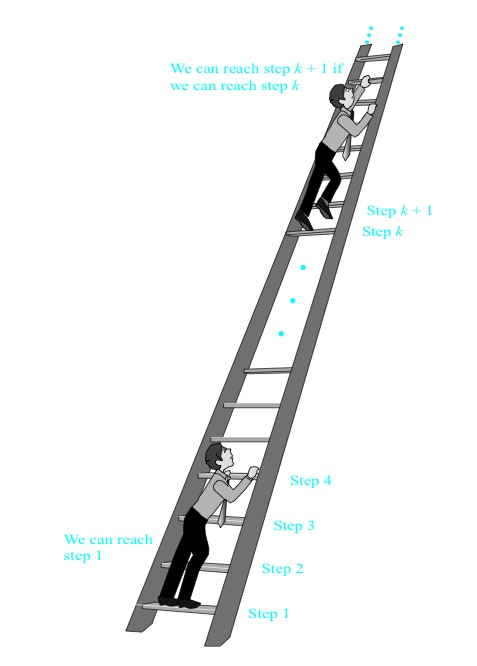
\includegraphics[height=8.8cm]{./img/lecture24-fig1.png}
     \end{column}
     \begin{column}[T]{7.5cm} % each column can also be its own environment
       \vspace{.3in}
       
       
       \Blue{ Motivation: Climbing an Infinite Ladder}
       \medskip
       
        
         Suppose we have an infinite ladder and the following capabilities:\\
         \medskip
         
         1. We can reach the first rung of the ladder.\\
         2. If we can reach a particular rung of the ladder, then we
	    can reach the next rung.
     

     \end{column}
    
     \end{columns}
     
\end{frame}

\begin{frame}[plain]{Principle of Mathematical Induction}
 \begin{itemize}
  \item Let $P(n)$ be a recurrence relation and $f(n)$ a hypersized closed-form formula. 
     The \Blue{Principle of Mathematical Induction} complete two steps to prove that $P(n)$
    is true for all $n\in\mathbb{Z}^+$: \pause 
   \begin{enumerate}
     \item {\bf Basis Step}: Show that $P(1)$ is true; that is, $P(1) = f(1)$.\pause 
     \item {\bf Inductive Step}: Let $k>1$ be some (unspecified) \Red{arbitrary}  integer.
        If $P(k) = f(k)$,  show that $P(k+1) = f(k+1)$.
        (In other wors, show that $P(k)\rightarrow P(k+1)$ is true for all $k\in \mathbb{Z}^+$.)\pause 
   \end{enumerate}
   Then, $P(n)$ is true for all $n\in \mathbb{Z}^+$.\pause 
    \item {\bf Remark:} Mathematical induction can be expressed as the rule of inference
   (here the domain is the set of all positive integers)
  \[ \Blue{ [P(1)\wedge \forall k [P(k)\rightarrow P(k+1)]] \rightarrow \forall n\, P(n) } \] 
 \end{itemize} 

\end{frame}

\begin{frame}[plain]{}

  {\bf Example 24.1}. Show that if $n$ is a positive integer, then
   \[ 1+2+3+ \cdots + n = \frac{n(n+1)}{2} \]
  
   \vspace{1.4in}

\end{frame}


\begin{frame}[plain]{Solution to Example 1}
 \begin{center}
  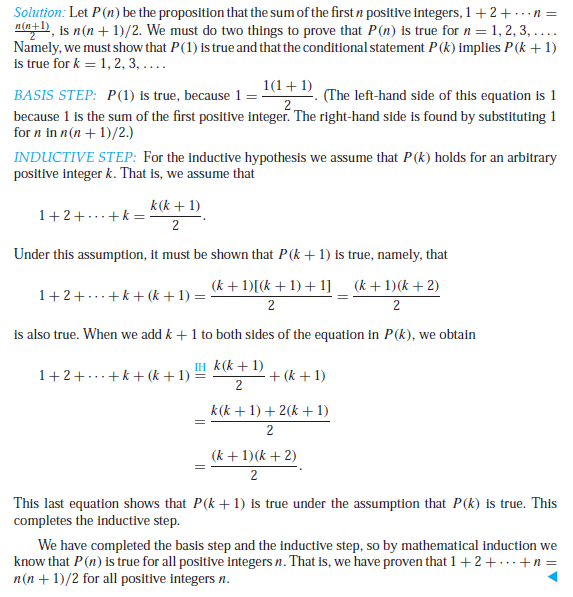
\includegraphics[height=7.5cm]{./img/lecture24-fig2.png}
 \end{center}

\end{frame}

\begin{frame}[plain]{}

   {\bf Practice 24.2}. Conjecture a formula for the sum of the first $n$
  positive odd integers. Then prove your conjecture using
   mathematical induction.
    \vspace{1.7in}
    

\end{frame}


\begin{frame}[plain]{}

{\bf Example 20.3}. The closed-form solution $f(n)$ for the recurrence relation 
    \[ H(n) = \left\{ \begin{array}{ccc}
                       1 &\mbox{if}& n = 1\\
                       H(n-1)+6n-6 &\mbox{if}& n>1
                      \end{array} \right. 
    \]
    %Essential, p190,  Example 3.10
 was 
  \[ f(n) = 3n^2-3n+1, \ \forall n = 1, 2, ...
  \]
  
  Use the mathematical induction to prove that $H(n) = f(n)$ for all $n\geq 1$.
  
  \vspace{1in}
   
 
\end{frame}




\end{document}%%%%%%%%%%%%%%%%%%%%%%%%%%%%%%%%%%%%%%%%%%%%%%%%%

